\section{Existing System: \idx{ScaleNet}} % (fold)
\label{sec:scalenet}

\idx{ScaleNet} \cite{SIE06} is a research project developed between 2005 and 2009.
Partly sponsored by the \emph{German Ministry of Education}, several major corporations participated, including \emph{Deutsche Telekom AG}, \emph{Alcatel SEL AG}, \emph{Eriksson GmbH}, \emph{Lucent Technologies} and \emph{Siemens AG}.
\ida{T-Labs} was specifically one of the departments more closely involved.

\begin{wrapfigure}{r}{0.5\textwidth}
  \centering
    
\includegraphics[width=0.48\textwidth]{logo-scalenet}
  \caption{\idx{ScaleNet} logo}
  \label{fig:logo-scalenet}
\end{wrapfigure}

The aim of \idx{ScaleNet} is to provide a \ida{NGN} that integrates different wireless and wireline access technologies.
It is advertised as a scalable, cost effective and efficient \ida{FMC} solution.

\subsection{System Overview} % (fold)
\label{sub:overviewscalenet}

\idx{ScaleNet} addresses both service and network convergence.
At the lower level, the system supports a multitude of heterogeneous physical and logical network elements of fixed and mobile networks into one single all-IP infrastructure.
Figure~\ref{fig:scalenet-structure} lists some of the protocols that could be used \cite{SIV08}.

\begin{figure}[htbp]
  \centering
    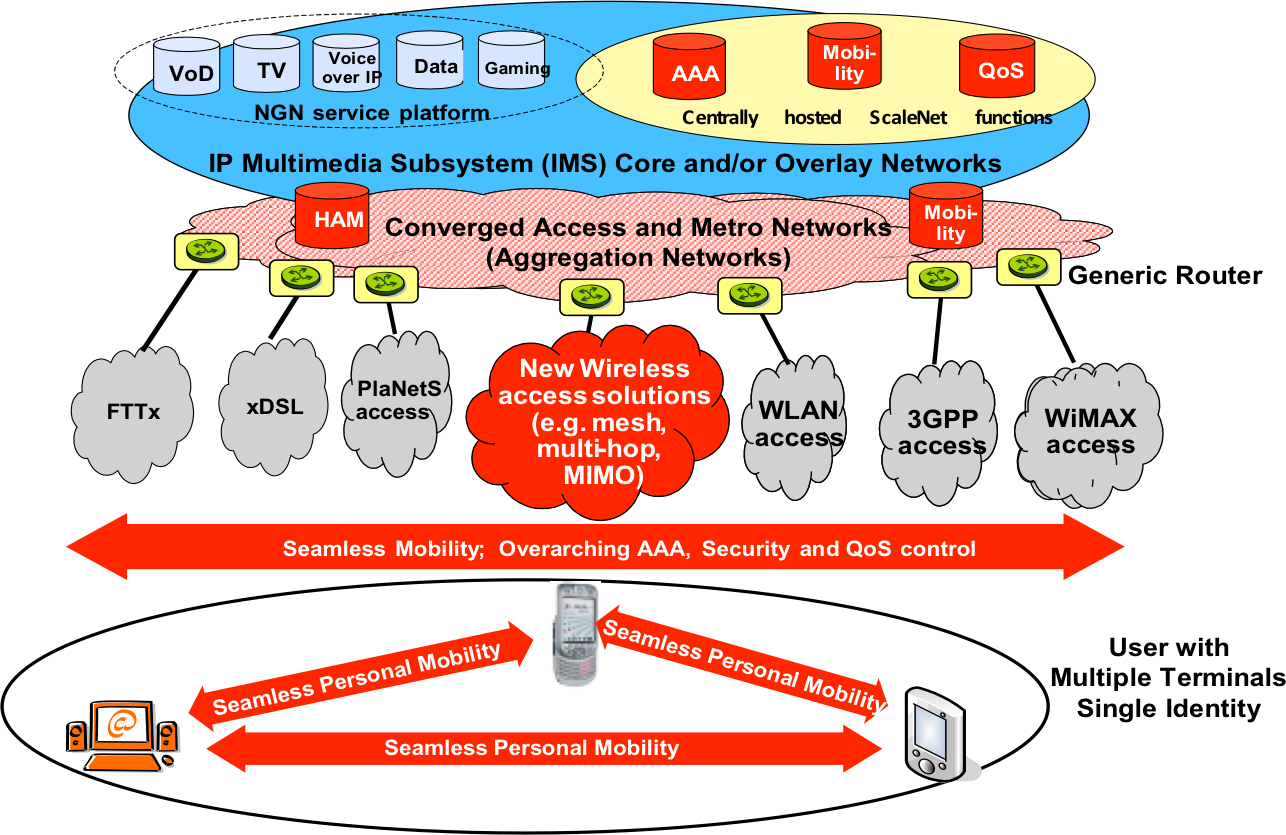
\includegraphics[width=\textwidth]{scalenet-structure}
  \caption{Structure of the system}
  \label{fig:scalenet-structure}
\end{figure}

At a upper level, multimedia services relay on the \ida{IMS} framework for the delivery.
Theoretically \idx{ScaleNet} could support other protocols like Overlay Networks or \ida{P2P}, but \ida{IMS} is the one used by the current implementation.

It is important to notice that the own network is user-centric, and transparently handles identities by using \ida{SIP}.
This eases handling users with multiple devices; therefore applications do not have to worry about that part.

It is also important to define what a session means in this system.
A session refers to the current use of a service, so for every service that the user is enjoying a session is created.
For example, if it is viewing a movie but also talking on the \ida{IP} phone, there are two sessions at the same time.

The creation of a session implies that a new service is created, but it goes the other way around too.
If a session is deleted, that service must stop.
If the user ends the service, the session must be deleted.
That means sessions have to be synchronized with the actual services.

A session is also linked to the device that the user is using.
The system allows the copy and transfer of sessions to other devices that he owns, wherever it makes sense.
Since the current implementation has also basic social capabilities, that session can also be transferred or copied to a user's contact.
In the context of this application a user's contact is called ``buddy''.
Figure~\ref{fig:scalenet-structure} lists some of the services that can be offered:

\begin{itemize}
  \item Voice \et{} Video Calls
  \item Mobile TV \et{} \ida{VOD}
  \item \index{MMOG}\acp{MMOG}
  \item Internet Access
\end{itemize}

The work described in this document is primarily focused on the second application, i.e., video streaming.
The idea is that the user can buy a video and play it anywhere using any supported device.

\nicesubsectionending

% subsection overviewscalenet (end)

\subsection{\idx{IMS} Demonstrator} % (fold)
\label{sub:demonstrator}

\begin{figure}[p]
  \centering
    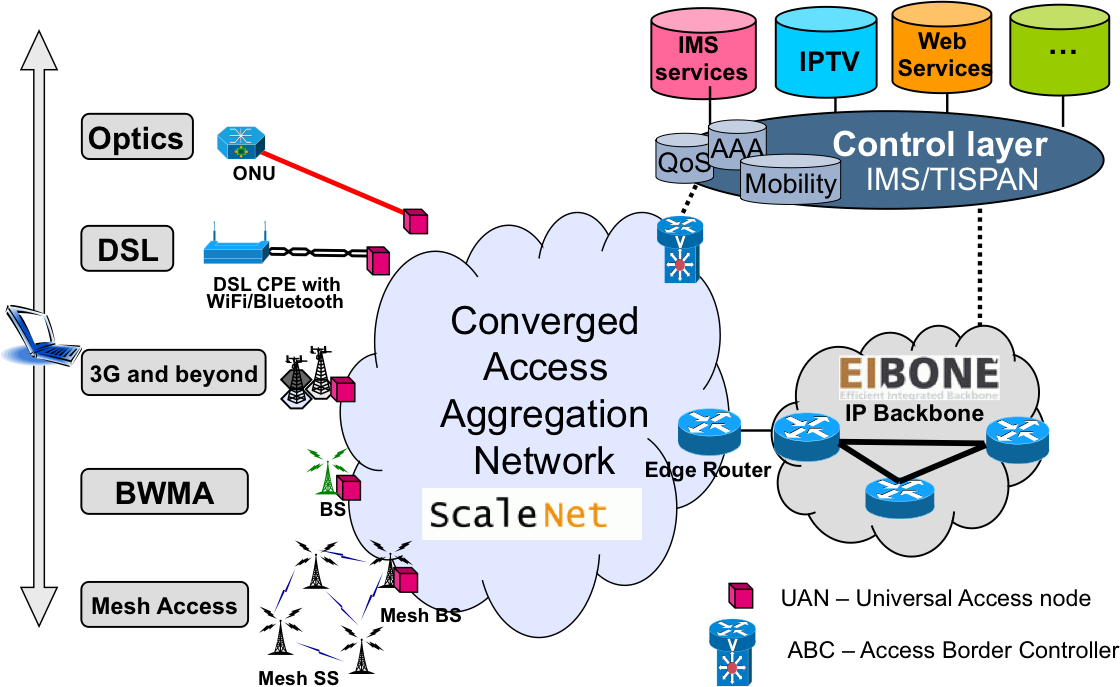
\includegraphics[width=\textwidth]{ims-arch}
  \caption{System architecture}
  \label{fig:ims-arch}
\end{figure}

\begin{figure}[p]
  \centering
    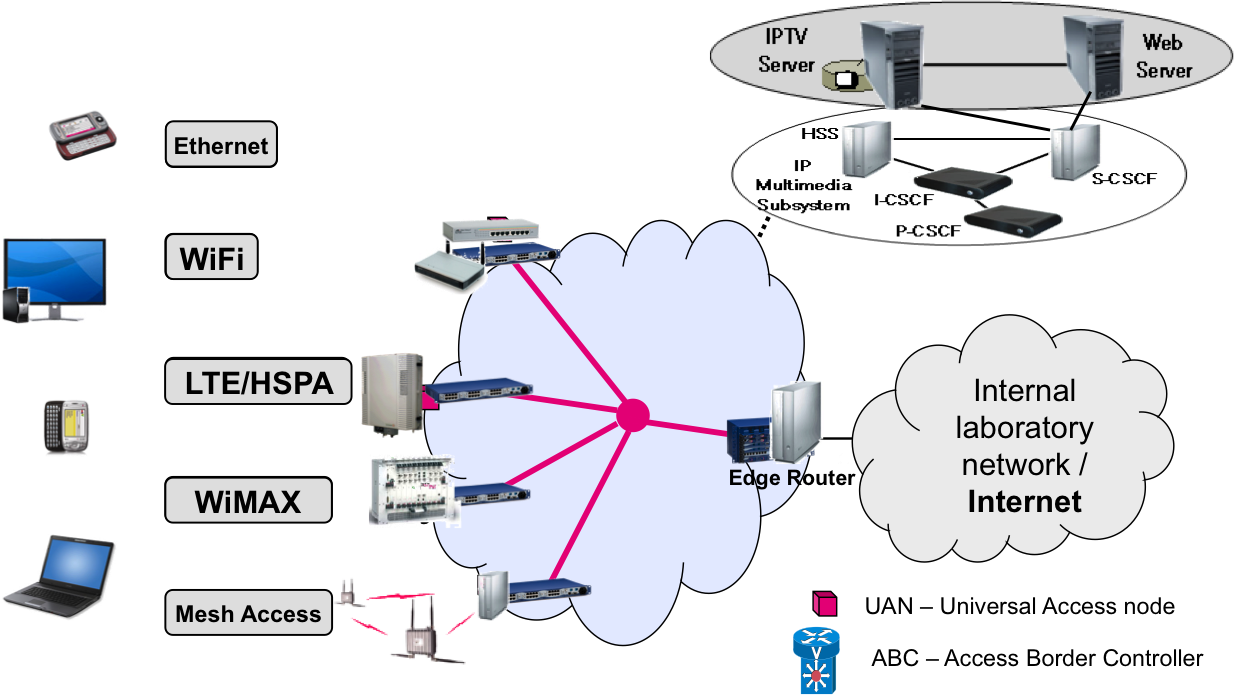
\includegraphics[width=\textwidth]{ims-arch-real}
  \caption{Architecture of the demonstrator}
  \label{fig:ims-arch-real}
\end{figure}

A logical view of the system is depicted in Figure~\ref{fig:ims-arch}, explaining the important nodes based on the capabilities needed.
The information relevant to this project is contained in the upper right corner of the figure, the nodes behind the control layer.

In the offices of \ida{T-Labs} in Berlin and Darmstadt there is a demonstrator with a working implementation of \idx{ScaleNet}.
That demonstrator is composed by several servers and a network infrastructure that enables access to the system using different network protocols and devices.
In Figure~\ref{fig:ims-arch-real} the actual network and hardware are exposed, replacing the same space as in the logical view (Figure~\ref{fig:ims-arch}).

\begin{figure}[htbp]
  \centering
    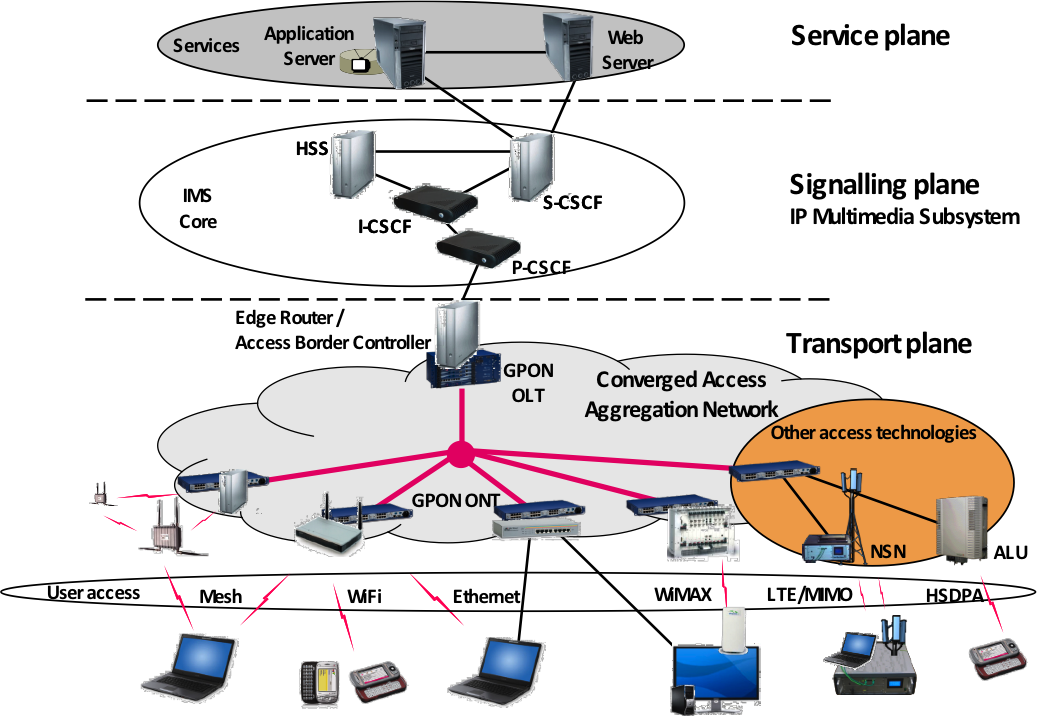
\includegraphics[width=\textwidth]{ims-setup}
  \caption{Setup of the demonstrator}
  \label{fig:ims-setup}
\end{figure}

Figure~\ref{fig:ims-setup} describes the setup in a better way and highlights the three different planes of the demonstrator.
The developed web application is executed from the \idx{Web Server} and the \idx{Application Server}, since it belongs to the service plane.
The signaling plane has also to be taken into account, because it communicates directly with the servers.

However, that is not the real deployment of the hardware used.
Whether for convenience or efficiency, tasks are distributed between two main servers.
This does not affect the logic of the system, since those tasks could be easily decoupled in an alternate deployment with more servers.
Anyway, the interesting pieces of hardware for this project are:

\begin{description}
  \item[\ida{IMS} core] This machine contains the \ida{IMS} server\footnote{The IMS core is open source software from Fraunhofer FOKUS and it can be freely downloaded from: \url{http://www.openimscore.org/}}, but since the \ida{IMS} load is not very high, it is responsible for other things.
  It acts as a \idx{Web Server} (using Apache Web Server\footnote{\url{http://httpd.apache.org/}}) serving \idas{PHP} applications.
  It is also the internal \idas{DNS} server.
  \item[\idx{Application Server}] This is the \idas{IPTV} server, where the video content is streamed.
  It is also a \idx{Web Server}, but it serves \idx{Java} applications based on the \idas{OSGi} framework\footnote{\url{http://www.osgi.org/}}.
  \item[User Devices] Devices intended for the user to access the services.
  There is a TV, a laptop and several phones.
  All of them run a custom \ida{IMS} client that holds a connection to the servers, allowing the identification and adding \idas{IPTV} and \idas{VoIP} capabilities to those devices.
  In the last phase of the development, an \idx{iPhone} was added for testing purposes.
\end{description}

This demonstrator contains several demo applications running.
The interesting one for this project is the application that handles \idas{IPTV} streaming.

\nicesubsectionending

% subsubsection stoppingplayback (end)

\subsection{Personal Network Administration Interface (\idx{PNAI})} % (fold)
\label{sub:pnai}

The Web interface used for the management of sessions is called \ida{PNAI}. From this interface the user can obtain this information:

\begin{itemize}
  \item All devices and registered in the system for that user and their online status.
  \item All buddies for that user and their online status.
  \item All multimedia sessions related to the user. This includes:
  \begin{itemize}
    \item The sessions running on his devices, no matter who paid for that content.
    \item The sessions running on devices from his buddies and started/paid by that user.
  \end{itemize}
\end{itemize}

Those are passive actions, but from that same view the user can initiate some operations to control the system.
In Figure~\ref{fig:usecasesiptv} all the available operations relating sessions are listed following a use case diagram.

\begin{figure}[htbp]
  \centering
    \includegraphics[width=\textwidth]{diagrams/usecases.1}
  \caption{Use cases for the IPTV application}
  \label{fig:usecasesiptv}
\end{figure}

In that diagram colors are used to differentiate the different kind of use cases covered. Also two visual marks (* and **) are added in case this is a copy in black a white. The meaning of the colors are explained according to this legend:

\begin{description}
  \item[Green] Available already in the main \ida{PNAI} page.
  \item[Purple (\emph{marked with *})] Available in an individual page outside of the main \ida{PNAI} page.
  \item[Red (\emph{marked with **})] Not implemented.
\end{description}

As we can see, the main \ida{PNAI} page has already a lot of functionality, but it can contain even more. Basically the actions available to that user in that page are:

\begin{itemize}
  \item Terminate a session of a user device or of a buddy if the session is owned by that user.
  \item Transfer (handover) or copy (duplication) a existing session to a user device or to a buddy if the session is owned by that user. That is, if one buddy bought the content for us, we cannot transfer again that content to another buddy.
\end{itemize}

Beside of these session related operations, there are other management operations.
For example, selecting which device is the default, adding/removing devices or adding/removing buddies.
For this document they are not relevant since they remained untouched.

Figure~\ref{fig:pnai-old} shows the old appearance of the main page for a logged user, before any work began.
On the left side of the page there is the \idx{Device List}, where the devices owned by that user are drawn.
On the right side there is the \idx{Buddy List}, where the user's buddies are listed.
Finally, the trash is in the lower right corner of the \idx{Device List}. 

\begin{figure}[htbp]
  \centering
    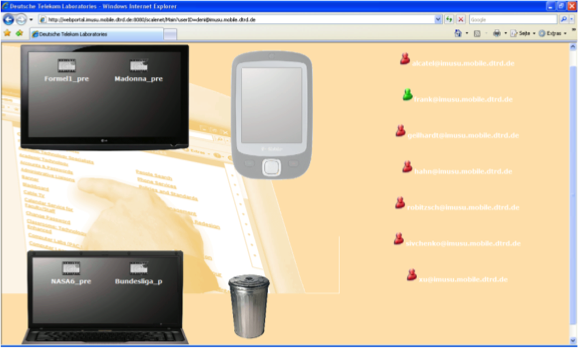
\includegraphics[width=\textwidth]{pnai-old}
  \caption{Old main \idas{PNAI} page}
  \label{fig:pnai-old}
\end{figure}

The devices that are offline are disabled and are drawn with a whitish appearance.
The buddies that are online are preceded by a green icon, while the ones that are offline are preceded by a red icon.

Devices or buddies that are online act as session containers. Inside of the 

\subsubsection{Use Cases} % (fold)
\label{ssub:usecasesold}

\begin{center}
  \begin{usecase}[Stop a session of a device]
    \label{tab:usecasestopdevice}%
    \usecaseactor{System user}
    \usecasepre{A session is already running on a device, and it is showing in the \ida{PNAI} interface inside of that device.}
    \usecasepost{Session must terminate, i.e., the content must stop playing. The user must be notified with a popup and the session icon must be deleted from the \ida{PNAI} interface.}
    \usecasemain{
      \begin{usecasepath}
        \item User starts dragging the session icon.
        \item A copy of the session icon appears under the user's cursor, and follows the cursor until the user drops it.
        \item User drops the cloned session icon into the trash.
        \item A popup appears to notify the user that the action is in progress and the cloned session icon is deleted from the view.
        \item The content stops playing.
        \item The popup disappears and the original session icon is deleted from the view.
      \end{usecasepath}
    }
    \usecasealt{1}{
      \begin{usecasepath}[b]
        \setcounter{enumi}{2}
        \item User drops the session into a blank space.
        \item Action is cancelled.
      \end{usecasepath}
    }
    \usecasealt{2}{
      \begin{usecasepath}[c]
        \setcounter{enumi}{4}
        \item There is an error with the server and the content keeps playing.
        \item The content of the popup changes to notify the user that there was an error with the server and the action could not be completed.
        After 5 seconds it disappears.
        \item Action is cancelled.
      \end{usecasepath}
    }
    \usecasealt{3}{
      \begin{usecasepath}[d]
        \item There is an error with the server and the content keeps playing.
        \item The content of the popup changes to notify the user that there was an error with the server and the action could not be completed.
        After 5 seconds it disappears.
        \item Action is cancelled.
      \end{usecasepath}
    }
  \end{usecase}
\end{center}

The use case for terminating a session that a buddy is playing and that we own is very similar:

\begin{center}
  \begin{usecase}[Stop a session of a buddy]
    \label{tab:usecasestopbuddy}%
    \usecaseactor{System user}
    \usecasepre{A session owned by the user is running on a device, and it is showing in the \ida{PNAI} interface near that buddy's name.}
    \usecasepost{Session must terminate, i.e., the content must stop playing. The user must be notified with a popup and the session icon must be deleted from the \ida{PNAI} interface. The buddy is \emph{not} notified, the content stops without warning.}
    \usecasemain{
      \begin{usecasepath}
        \item User starts dragging the session icon.
        \item A copy of the session icon appears under the user's cursor, and follows the cursor until the user drops it.
        \item User drops the cloned session icon into the trash.
        \item A popup appears to notify the user that the action is in progress and the cloned session icon is deleted from the view.
        \item The content stops playing.
        \item The popup disappears and the original session icon is deleted from the view.
      \end{usecasepath}
    }
    \usecasealt{1}{
      \begin{usecasepath}[b]
        \setcounter{enumi}{2}
        \item User drops the session into a blank space.
        \item Action is cancelled.
      \end{usecasepath}
    }
    \usecasealt{2}{
      \begin{usecasepath}[c]
        \setcounter{enumi}{4}
        \item There is an error with the server and the content keeps playing.
        \item The content of the popup changes to notify the user that there was an error with the server and the action could not be completed.
        After 5 seconds it disappears.
        \item Action is cancelled.
      \end{usecasepath}
    }
  \end{usecase}
\end{center}

% subsubsection usecasesold (end)


% subsection pnai (end)

% section scalenet (end)
